\documentclass[12pt,aspectratio=1610]{ecnubeamerformyself}

% Override image paths (set here so the .cls keeps defaults)
% \renewcommand{\ECNUBackgroundImage}{img/bg.pdf}
% \renewcommand{\ECNUFrameLogoImage}{img/logo-white.pdf}
% \renewcommand{\ECNUFirstPageBG}{img/firstpagebg.jpg}
% \renewcommand{\ECNUMathLogo}{img/math-logo.pdf}
% \renewcommand{\ECNULibThanks}{img/lib.png}

\addbibresource{../ref.bib}
%一些常用的宏定义
\newcommand{\bbA}{{\mathbb{A}}}
\newcommand{\bba}{{\mathbb{a}}}
\newcommand{\bbB}{{\mathbb{B}}}
\newcommand{\bbb}{{\mathbb{b}}}
\newcommand{\bbC}{{\mathbb{C}}}
\newcommand{\bbc}{{\mathbb{c}}}
\newcommand{\bbD}{{\mathbb{D}}} 
\newcommand{\bbd}{{\mathbb{d}}}
\newcommand{\bbE}{{\mathbb{E}}}
\newcommand{\bbe}{{\mathbb{e}}}
\newcommand{\bbF}{{\mathbb{F}}}
\newcommand{\bbf}{{\mathbb{f}}}
\newcommand{\bbG}{{\mathbb{G}}}
\newcommand{\bbg}{{\mathbb{g}}}
\newcommand{\bbH}{{\mathbb{H}}}
\newcommand{\bbh}{{\mathbb{h}}}
\newcommand{\bbI}{{\mathbb{I}}}
\newcommand{\bbi}{{\mathbb{i}}}
\newcommand{\bbJ}{{\mathbb{J}}}
\newcommand{\bbj}{{\mathbb{j}}}
\newcommand{\bbK}{{\mathbb{K}}}
\newcommand{\bbk}{{\mathbb{k}}}
\newcommand{\bbL}{{\mathbb{L}}}
\newcommand{\bbl}{{\mathbb{l}}}
\newcommand{\bbM}{{\mathbb{M}}}
\newcommand{\bbm}{{\mathbb{m}}}
\newcommand{\bbN}{{\mathbb{N}}}
\newcommand{\bbn}{{\mathbb{n}}}
\newcommand{\bbO}{{\mathbb{O}}}
\newcommand{\bbo}{{\mathbb{o}}}
\newcommand{\bbP}{{\mathbb{P}}}
\newcommand{\bbp}{{\mathbb{p}}}
\newcommand{\bbQ}{{\mathbb{Q}}}
\newcommand{\bbq}{{\mathbb{q}}}
\newcommand{\bbR}{{\mathbb{R}}}
\newcommand{\bbr}{{\mathbb{r}}}
\newcommand{\bbS}{{\mathbb{S}}}
\newcommand{\bbs}{{\mathbb{s}}}
\newcommand{\bbT}{{\mathbb{T}}}
\newcommand{\bbt}{{\mathbb{t}}}
\newcommand{\bbU}{{\mathbb{U}}}
\newcommand{\bbu}{{\mathbb{u}}}
\newcommand{\bbV}{{\mathbb{V}}}
\newcommand{\bbv}{{\mathbb{v}}}
\newcommand{\bbW}{{\mathbb{W}}}
\newcommand{\bbw}{{\mathbb{w}}}
\newcommand{\bbX}{{\mathbb{X}}}
\newcommand{\bbx}{{\mathbb{x}}}
\newcommand{\bbY}{{\mathbb{Y}}}
\newcommand{\bby}{{\mathbb{y}}}
\newcommand{\bbZ}{{\mathbb{Z}}}
\newcommand{\bbz}{{\mathbb{z}}}
\newcommand{\bbone}{{\mathbb{1}}}

\newcommand{\calA}{{\mathcal{A}}}
\newcommand{\cala}{{\mathcal{a}}}
\newcommand{\calB}{{\mathcal{B}}}
\newcommand{\calb}{{\mathcal{b}}}
\newcommand{\calC}{{\mathcal{C}}}
\newcommand{\calc}{{\mathcal{c}}}
\newcommand{\calD}{{\mathcal{D}}}
\newcommand{\cald}{{\mathcal{d}}}
\newcommand{\calE}{{\mathcal{E}}}
\newcommand{\cale}{{\mathcal{e}}}
\newcommand{\calF}{{\mathcal{F}}}
\newcommand{\calf}{{\mathcal{f}}}
\newcommand{\calG}{{\mathcal{G}}}
\newcommand{\calg}{{\mathcal{g}}}
\newcommand{\calH}{{\mathcal{H}}}
\newcommand{\calh}{{\mathcal{h}}}
\newcommand{\calI}{{\mathcal{I}}}
\newcommand{\cali}{{\mathcal{i}}}
\newcommand{\calJ}{{\mathcal{J}}}
\newcommand{\calj}{{\mathcal{j}}}
\newcommand{\calK}{{\mathcal{K}}}
\newcommand{\calk}{{\mathcal{k}}}
\newcommand{\calL}{{\mathcal{L}}}
\newcommand{\call}{{\mathcal{l}}}
\newcommand{\calM}{{\mathcal{M}}}
\newcommand{\calm}{{\mathcal{m}}}
\newcommand{\calN}{{\mathcal{N}}}
\newcommand{\caln}{{\mathcal{n}}}
\newcommand{\calO}{{\mathcal{O}}}
\newcommand{\calo}{{\mathcal{o}}}
\newcommand{\calP}{{\mathcal{P}}}
\newcommand{\calp}{{\mathcal{p}}}
\newcommand{\calQ}{{\mathcal{Q}}}
\newcommand{\calq}{{\mathcal{q}}}
\newcommand{\calR}{{\mathcal{R}}}
\newcommand{\calr}{{\mathcal{r}}}
\newcommand{\calS}{{\mathcal{S}}}
\newcommand{\cals}{{\mathcal{s}}}
\newcommand{\calT}{{\mathcal{T}}}
\newcommand{\calt}{{\mathcal{t}}}
\newcommand{\calU}{{\mathcal{U}}}
\newcommand{\calu}{{\mathcal{u}}}
\newcommand{\calV}{{\mathcal{V}}}
\newcommand{\calv}{{\mathcal{v}}}
\newcommand{\calW}{{\mathcal{W}}}
\newcommand{\calw}{{\mathcal{w}}}
\newcommand{\calX}{{\mathcal{X}}}
\newcommand{\calx}{{\mathcal{x}}}
\newcommand{\calY}{{\mathcal{Y}}}
\newcommand{\caly}{{\mathcal{y}}}
\newcommand{\calZ}{{\mathcal{Z}}}
\newcommand{\calz}{{\mathcal{z}}}

\newcommand{\frakA}{{\mathfrak{A}}}
\newcommand{\fraka}{{\mathfrak{a}}}
\newcommand{\frakB}{{\mathfrak{B}}}
\newcommand{\frakb}{{\mathfrak{b}}}
\newcommand{\frakC}{{\mathfrak{C}}}
\newcommand{\frakc}{{\mathfrak{c}}}
\newcommand{\frakD}{{\mathfrak{D}}}
\newcommand{\frakd}{{\mathfrak{d}}}
\newcommand{\frakE}{{\mathfrak{E}}}
\newcommand{\frake}{{\mathfrak{e}}}
\newcommand{\frakF}{{\mathfrak{F}}}
\newcommand{\frakf}{{\mathfrak{f}}}
\newcommand{\frakG}{{\mathfrak{G}}}
\newcommand{\frakg}{{\mathfrak{g}}}
\newcommand{\frakH}{{\mathfrak{H}}}
\newcommand{\frakh}{{\mathfrak{h}}}
\newcommand{\frakI}{{\mathfrak{I}}}
\newcommand{\fraki}{{\mathfrak{i}}}
\newcommand{\frakJ}{{\mathfrak{J}}}
\newcommand{\frakj}{{\mathfrak{j}}}
\newcommand{\frakK}{{\mathfrak{K}}}
\newcommand{\frakk}{{\mathfrak{k}}}
\newcommand{\frakL}{{\mathfrak{L}}}
\newcommand{\frakl}{{\mathfrak{l}}}
\newcommand{\frakM}{{\mathfrak{M}}}
\newcommand{\frakm}{{\mathfrak{m}}}
\newcommand{\frakN}{{\mathfrak{N}}}
\newcommand{\frakn}{{\mathfrak{n}}}
\newcommand{\frakO}{{\mathfrak{O}}}
\newcommand{\frako}{{\mathfrak{o}}}
\newcommand{\frakP}{{\mathfrak{P}}}
\newcommand{\frakp}{{\mathfrak{p}}}
\newcommand{\frakQ}{{\mathfrak{Q}}}
\newcommand{\frakq}{{\mathfrak{q}}}
\newcommand{\frakR}{{\mathfrak{R}}}
\newcommand{\frakr}{{\mathfrak{r}}}
\newcommand{\frakS}{{\mathfrak{S}}}
\newcommand{\fraks}{{\mathfrak{s}}}
\newcommand{\frakT}{{\mathfrak{T}}}
\newcommand{\frakt}{{\mathfrak{t}}}
\newcommand{\frakU}{{\mathfrak{U}}}
\newcommand{\fraku}{{\mathfrak{u}}}
\newcommand{\frakV}{{\mathfrak{V}}}
\newcommand{\frakv}{{\mathfrak{v}}}
\newcommand{\frakW}{{\mathfrak{W}}}
\newcommand{\frakw}{{\mathfrak{w}}}
\newcommand{\frakX}{{\mathfrak{X}}}
\newcommand{\frakx}{{\mathfrak{x}}}
\newcommand{\frakY}{{\mathfrak{Y}}}
\newcommand{\fraky}{{\mathfrak{y}}}
\newcommand{\frakZ}{{\mathfrak{Z}}}
\newcommand{\frakz}{{\mathfrak{z}}}

\newcommand{\rmA}{{\mathrm{A}}}
\newcommand{\rma}{{\mathrm{a}}}
\newcommand{\rmB}{{\mathrm{B}}}
\newcommand{\rmb}{{\mathrm{b}}}
\newcommand{\rmC}{{\mathrm{C}}}
\newcommand{\rmc}{{\mathrm{c}}}
\newcommand{\rmD}{{\mathrm{D}}}
\newcommand{\rmd}{{\mathrm{d}}}
\newcommand{\rmE}{{\mathrm{E}}}
\newcommand{\rme}{{\mathrm{e}}}
\newcommand{\rmF}{{\mathrm{F}}}
\newcommand{\rmf}{{\mathrm{f}}}
\newcommand{\rmG}{{\mathrm{G}}}
\newcommand{\rmg}{{\mathrm{g}}}
\newcommand{\rmH}{{\mathrm{H}}}
\newcommand{\rmh}{{\mathrm{h}}}
\newcommand{\rmI}{{\mathrm{I}}}
\newcommand{\rmi}{{\mathrm{i}}}
\newcommand{\rmJ}{{\mathrm{J}}}
\newcommand{\rmj}{{\mathrm{j}}}
\newcommand{\rmK}{{\mathrm{K}}}
\newcommand{\rmk}{{\mathrm{k}}}
\newcommand{\rmL}{{\mathrm{L}}}
\newcommand{\rml}{{\mathrm{l}}}
\newcommand{\rmM}{{\mathrm{M}}}
\newcommand{\rmm}{{\mathrm{m}}}
\newcommand{\rmN}{{\mathrm{N}}}
\newcommand{\rmn}{{\mathrm{n}}}
\newcommand{\rmO}{{\mathrm{O}}}
\newcommand{\rmo}{{\mathrm{o}}}
\newcommand{\rmP}{{\mathrm{P}}}
\newcommand{\rmp}{{\mathrm{p}}}
\newcommand{\rmQ}{{\mathrm{Q}}}
\newcommand{\rmq}{{\mathrm{q}}}
\newcommand{\rmR}{{\mathrm{R}}}
\newcommand{\rmr}{{\mathrm{r}}}
\newcommand{\rmS}{{\mathrm{S}}}
\newcommand{\rms}{{\mathrm{s}}}
\newcommand{\rmT}{{\mathrm{T}}}
\newcommand{\rmt}{{\mathrm{t}}}
\newcommand{\rmU}{{\mathrm{U}}}
\newcommand{\rmu}{{\mathrm{u}}}
\newcommand{\rmV}{{\mathrm{V}}}
\newcommand{\rmv}{{\mathrm{v}}}
\newcommand{\rmW}{{\mathrm{W}}}
\newcommand{\rmw}{{\mathrm{w}}}
\newcommand{\rmX}{{\mathrm{X}}}
\newcommand{\rmx}{{\mathrm{x}}}
\newcommand{\rmY}{{\mathrm{Y}}}
\newcommand{\rmy}{{\mathrm{y}}}
\newcommand{\rmZ}{{\mathrm{Z}}}

\newcommand{\bfA}{{\mathbf{A}}}
\newcommand{\bfa}{{\mathbf{a}}}
\newcommand{\bfB}{{\mathbf{B}}}
\newcommand{\bfb}{{\mathbf{b}}}
\newcommand{\bfC}{{\mathbf{C}}}
\newcommand{\bfc}{{\mathbf{c}}}
\newcommand{\bfD}{{\mathbf{D}}}
\newcommand{\bfd}{{\mathbf{d}}}
\newcommand{\bfE}{{\mathbf{E}}}
\newcommand{\bfe}{{\mathbf{e}}}
\newcommand{\bfF}{{\mathbf{F}}}
\newcommand{\bff}{{\mathbf{f}}}
\newcommand{\bfG}{{\mathbf{G}}}
\newcommand{\bfg}{{\mathbf{g}}}
\newcommand{\bfH}{{\mathbf{H}}}
\newcommand{\bfh}{{\mathbf{h}}}
\newcommand{\bfI}{{\mathbf{I}}}
\newcommand{\bfi}{{\mathbf{i}}}
\newcommand{\bfJ}{{\mathbf{J}}}
\newcommand{\bfj}{{\mathbf{j}}}
\newcommand{\bfK}{{\mathbf{K}}}
\newcommand{\bfk}{{\mathbf{k}}}
\newcommand{\bfL}{{\mathbf{L}}}
\newcommand{\bfl}{{\mathbf{l}}}
\newcommand{\bfM}{{\mathbf{M}}}
\newcommand{\bfm}{{\mathbf{m}}}
\newcommand{\bfN}{{\mathbf{N}}}
\newcommand{\bfn}{{\mathbf{n}}}
\newcommand{\bfO}{{\mathbf{O}}}
\newcommand{\bfo}{{\mathbf{o}}}
\newcommand{\bfP}{{\mathbf{P}}}
\newcommand{\bfp}{{\mathbf{p}}}
\newcommand{\bfQ}{{\mathbf{Q}}}
\newcommand{\bfq}{{\mathbf{q}}}
\newcommand{\bfR}{{\mathbf{R}}}
\newcommand{\bfr}{{\mathbf{r}}}
\newcommand{\bfS}{{\mathbf{S}}}
\newcommand{\bfs}{{\mathbf{s}}}
\newcommand{\bfT}{{\mathbf{T}}}
\newcommand{\bft}{{\mathbf{t}}}
\newcommand{\bfU}{{\mathbf{U}}}
\newcommand{\bfu}{{\mathbf{u}}}
\newcommand{\bfV}{{\mathbf{V}}}
\newcommand{\bfv}{{\mathbf{v}}}
\newcommand{\bfW}{{\mathbf{W}}}
\newcommand{\bfw}{{\mathbf{w}}}
\newcommand{\bfX}{{\mathbf{X}}}
\newcommand{\bfx}{{\mathbf{x}}}
\newcommand{\bfY}{{\mathbf{Y}}}
\newcommand{\bfy}{{\mathbf{y}}}
\newcommand{\bfZ}{{\mathbf{Z}}}
\newcommand{\bfz}{{\mathbf{z}}}

\newcommand{\sfA}{{\mathsf{A}}}
\newcommand{\sfa}{{\mathsf{a}}}
\newcommand{\sfB}{{\mathsf{B}}}
\newcommand{\sfb}{{\mathsf{b}}}
\newcommand{\sfC}{{\mathsf{C}}}
\newcommand{\sfc}{{\mathsf{c}}}
\newcommand{\sfD}{{\mathsf{D}}}
\newcommand{\sfd}{{\mathsf{d}}}
\newcommand{\sfE}{{\mathsf{E}}}
\newcommand{\sfe}{{\mathsf{e}}}
\newcommand{\sfF}{{\mathsf{F}}}
\newcommand{\sff}{{\mathsf{f}}}
\newcommand{\sfG}{{\mathsf{G}}}
\newcommand{\sfg}{{\mathsf{g}}}
\newcommand{\sfH}{{\mathsf{H}}}
\newcommand{\sfh}{{\mathsf{h}}}
\newcommand{\sfI}{{\mathsf{I}}}
\newcommand{\sfi}{{\mathsf{i}}}
\newcommand{\sfJ}{{\mathsf{J}}}
\newcommand{\sfj}{{\mathsf{j}}}
\newcommand{\sfK}{{\mathsf{K}}}
\newcommand{\sfk}{{\mathsf{k}}}
\newcommand{\sfL}{{\mathsf{L}}}
\newcommand{\sfl}{{\mathsf{l}}}
\newcommand{\sfM}{{\mathsf{M}}}
\newcommand{\sfm}{{\mathsf{m}}}
\newcommand{\sfN}{{\mathsf{N}}}
\newcommand{\sfn}{{\mathsf{n}}}
\newcommand{\sfO}{{\mathsf{O}}}
\newcommand{\sfo}{{\mathsf{o}}}
\newcommand{\sfP}{{\mathsf{P}}}
\newcommand{\sfp}{{\mathsf{p}}}
\newcommand{\sfQ}{{\mathsf{Q}}}
\newcommand{\sfq}{{\mathsf{q}}}
\newcommand{\sfR}{{\mathsf{R}}}
\newcommand{\sfr}{{\mathsf{r}}}
\newcommand{\sfS}{{\mathsf{S}}}
\newcommand{\sfs}{{\mathsf{s}}}
\newcommand{\sfT}{{\mathsf{T}}}
\newcommand{\sft}{{\mathsf{t}}}
\newcommand{\sfU}{{\mathsf{U}}}
\newcommand{\sfu}{{\mathsf{u}}}
\newcommand{\sfV}{{\mathsf{V}}}
\newcommand{\sfv}{{\mathsf{v}}}
\newcommand{\sfW}{{\mathsf{W}}}
\newcommand{\sfw}{{\mathsf{w}}}
\newcommand{\sfX}{{\mathsf{X}}}
\newcommand{\sfx}{{\mathsf{x}}}
\newcommand{\sfY}{{\mathsf{Y}}}
\newcommand{\sfy}{{\mathsf{y}}}
\newcommand{\sfZ}{{\mathsf{Z}}}
\newcommand{\sfz}{{\mathsf{z}}}


\newcommand{\kk}{{\mathbf{k}}}
\newcommand{\kkk}{{\mathbb{k}}}
\newcommand{\KK}{{\mathbf{K}}}
\newcommand{\KKK}{{\mathbb{K}}}
\newcommand{\rkk}{{\kappa}} % residue field
\newcommand{\fkk}{{\mathscr{K}}} % fraction field

\renewcommand{\d}{{\mathrm{d}}}
\renewcommand{\i}{{\mathrm{i}}}
\renewcommand{\P}{\partial}


\newcommand{\Set}{\mathbf{Set}}
\newcommand{\Var}{\mathbf{Var}}
\newcommand{\Sch}{\mathbf{Sch}}
\newcommand{\Alg}{\mathbf{Alg}}
\newcommand{\Ring}{\mathbf{Ring}}
\newcommand{\Mod}{\mathbf{Mod}}
\newcommand{\TopMod}{\mathbf{TopMod}}
\newcommand{\Grp}{\mathbf{Grp}}
\newcommand{\Ab}{\mathbf{Ab}}
\newcommand{\Top}{\mathbf{Top}}
\newcommand{\Cat}{\mathbf{Cat}}
\newcommand{\AlgSp}{\mathbf{AlgSp}}
\newcommand{\Obj}{\operatorname{Obj}}


\newcommand{\ten}{\otimes}
\newcommand{\ratmap}{\dasharrow}
\newcommand{\injmap}{\hookrightarrow}
\newcommand{\surjmap}{\twoheadrightarrow}

\newcommand{\id}{{\operatorname{id}}}

\newcommand{\Frac}{\operatorname{Frac}}
\newcommand{\Der}{\operatorname{Der}}
\newcommand{\Spec}{\operatorname{Spec}}
\newcommand{\spec}{\operatorname{Spec}}
\newcommand{\mSpec}{\operatorname{mSpec}}
\newcommand{\depth}{\operatorname{depth}}
\newcommand{\idealht}{\operatorname{ht}}
\newcommand{\codim}{\operatorname{codim}}
\newcommand{\Supp}{\operatorname{Supp}}
\newcommand{\trdeg}{\operatorname{trdeg}}
\newcommand{\Ass}{\operatorname{Ass}}
\newcommand{\Ann}{\operatorname{Ann}}
\newcommand{\Ext}{\operatorname{Ext}}
\newcommand{\Tor}{\operatorname{Tor}}
\newcommand{\Hom}{\operatorname{Hom}}
\newcommand{\Eq}{\operatorname{Eq}}
\newcommand{\End}{\operatorname{End}}
\newcommand{\Mor}{\operatorname{Mor}}
\newcommand{\Mult}{\operatorname{Mult}}
\renewcommand{\Im}{\operatorname{Im}}
\newcommand{\Ker}{\operatorname{Ker}}
\newcommand{\rank}{\operatorname{rank}}
\newcommand{\cohdim}{\operatorname{coh.dim}}
\newcommand{\hldim}{\operatorname{hl.dim}}
\newcommand{\projdim}{\operatorname{proj.dim}}
\newcommand{\injdim}{\operatorname{inj.dim}}
\newcommand{\rad}{\operatorname{rad}}
\newcommand{\nil}{\operatorname{nil}}
\newcommand{\characteristic}{\operatorname{char}}
\newcommand{\Pic}{\operatorname{Pic}}
\newcommand{\NS}{\operatorname{NS}}
\newcommand{\Exc}{\operatorname{Exc}}
\newcommand{\Sing}{\operatorname{Sing}}
\newcommand{\Reg}{\operatorname{Reg}}
\newcommand{\Tr}{\operatorname{Tr}}
\newcommand{\Psef}{\operatorname{Psef}}
\newcommand{\Nef}{\operatorname{Nef}}
\newcommand{\Amp}{\operatorname{Amp}}
\newcommand{\Bigcone}{\operatorname{Big}}
\newcommand{\Frob}{\operatorname{Frob}}
\newcommand{\Bs}{\operatorname{Bs}}
\newcommand{\Stab}{\operatorname{Stab}}
\newcommand{\Sp}{\operatorname{Sp}}


\newcommand{\calHom}{{\mathcal{H\!o\!m}}}
\newcommand{\calExt}{{\mathcal{Ext}}}
\newcommand{\calProj}{{\mathcal{P\!r\!o\!j}}}
\newcommand{\calSpec}{{\mathcal{S\!p\!e\!c}}}


\newcommand{\mat}[4]{\left[ \begin{array}{cc}#1 &#2 \\ #3 &#4\end{array}\right]}
\newcommand{\threemat}[9]{\left[ \begin{array}{ccc}
  #1 & #2 & #3 \\
  #4 & #5 & #6 \\
  #7 & #8 & #9
\end{array}\right]}
\newcommand{\genmat}[9]{\left( \begin{array}{cccc}
  #1 & #2 & \cdots & #3 \\
  #4 & #5 & \cdots & #6 \\  
  \ldots & \ldots & \ddots & \ldots \\
  #7 & #8 & \cdots & #9
\end{array}\right)}





\newcommand{\contradiction}{
    \raisebox{-0.6ex}{\makebox[2.4ex][c]{
\begin{tikzpicture}
        \draw (0,0) circle (1.2ex);
        \draw (0.7 ex, 0.7 ex) -- (-0.4 ex, 0.7 ex);
        \draw (-0.4 ex, 0.7 ex) -- (0.7 ex, -0.4 ex);
        \draw (0.7 ex, -0.4 ex) -- (0.7 ex, 0.7 ex);
        \draw (0.7 ex, 0.7 ex) -- (-0.848 ex, -0.848 ex);
    \end{tikzpicture}}}
    \ \ 
}

% legendre符号
\makeatletter
\def\legendre@dash#1#2{\hb@xt@#1{%
  \kern-#2\p@
  \cleaders\hbox{\kern.5\p@
    \vrule\@height.2\p@\@depth.2\p@\@width\p@
    \kern.5\p@}\hfil
  \kern-#2\p@
  }}
\def\@legendre#1#2#3#4#5{\mathopen{}\left(
  \sbox\z@{$\genfrac{}{}{0pt}{#1}{#3#4}{#3#5}$}%
  \dimen@=\wd\z@
  \kern-\p@\vcenter{\box0}\kern-\dimen@\vcenter{\legendre@dash\dimen@{#2}}\kern-\p@
  \right)\mathclose{}}
\newcommand\legendre[2]{\mathchoice
  {\@legendre{0}{1}{}{#1}{#2}}
  {\@legendre{1}{.5}{\vphantom{1}}{#1}{#2}}
  {\@legendre{2}{0}{\vphantom{1}}{#1}{#2}}
  {\@legendre{3}{0}{\vphantom{1}}{#1}{#2}}
}
\def\dlegendre{\@legendre{0}{1}{}}
\def\tlegendre{\@legendre{1}{0.5}{\vphantom{1}}}
\makeatother
\usepackage{tikz-cd}
\usetikzlibrary{arrows.meta,calc,positioning}
\usepackage{pifont}  % 提供 \ding 命令

\def\acts{\ \rotatebox[origin=c]{-90}{$\circlearrowright$}\ }
\def\racts{\ \rotatebox[origin=c]{90}{$\circlearrowleft$}\ }
% \def\dacts{\ \rotatebox[origin=c]{0}{$\circlearrowright$}\ }
% \def\uacts{\ \rotatebox[origin=c]{180}{$\circlearrowright$}\ }

\title{Algebraic Dynamics and Dynamical Iitaka Theory}
% \subtitle{}
\date{Undergraduate Forum, ICCM 2025, January 7, 2026}
\author{{\Large Tianle Yang} \texorpdfstring{\\}{,} based on the joint work with Sheng Meng and Long Wang}


% Institute logo on the title page
\titlegraphic{\hfill\includegraphics[height=1.2cm]{\ECNUMathLogo}}


\begin{document}

% First page with different background
{
    \setbeamertemplate{background}{
        \includegraphics[width=\paperwidth,height=\paperheight]{\ECNUFirstPageBG}
    }
    \maketitle
}


% ----------------------------------------------------------


\begin{frame}{Kawaguchi-Silverman Conjecture}

    \vspace{0.3em}
        
    % \(/\overline{\bbQ}\). \(X\) smooth projective variety; \(f:X \to X\) surjective endomorphism.
    % Let \(X\) be a smooth projective variety over \(\overline{\bbQ}\) and \(f:X \to X\) a surjective endomorphism.
    % Smooth projective variety \(X / \overline{\bbQ}\); surjective endomorphism \(f:X \to X\).
    % Fix an ample line bundle \(H\) and a height function \(h\geq 1\) associated to \(H\).
    Setup: \(X\) sm. proj. var. \(/\overline{\bbQ}\); \(f:X \to X\) surj. endo.; \(H\) ample l.b.;\\ \(h \geq 1\) height function ass. to \(H\).

    \pause
    \vspace{0.2em}

    \begin{conjecture}[{Kawaguchi-Silverman Conjecture $=$ KSC}]\label{conj: ksc} 
        If the orbit \(O_f(x):=\{f^n(x)\,|\,n\ge 0\}\) is Zariski dense in \(X\), then 
        % the dynamical degree equals the arithmetic degree, i.e.,
        \[ \textcolor<3->{cyan}{\delta_f} = \textcolor<4->{magenta}{\alpha_f(x)}. \]
    \end{conjecture} 

    % \pause
    \vspace{-0.2em}


    % \vspace{0.5em}
    \begin{center}
    \begin{tabular}{cll}
        \visible<3->{
            \textbullet & \textcolor{cyan}{dynamical degree}: & \\
                & \(\displaystyle \textcolor{cyan}{\delta_f} := \lim_{n\to\infty} ((f^n)^*H \cdot H^{\dim X - 1})^{\frac{1}{n}}\) 
                & a \textcolor{cyan}{geometric, global} invariant of \(f\). \\
        }
        \visible<4->{
            \textbullet & \textcolor{magenta}{arithmetic degree}: & \\
                & \(\displaystyle \textcolor{magenta}{\alpha_f(x)} := \lim_{n\to\infty} h(f^n(x))^{\frac{1}{n}}\)
                & an \textcolor{magenta}{arithmetic, local} invariant at \(x\); \\
        }
    \end{tabular}
    \end{center}

    \vspace{-0.7cm}
    \visible<5->{
        \begin{center}
            \textbf{Slogan:} {\Large\textcolor{cyan}{GEOMETRY}} controls {\Large\textcolor{magenta}{ARITHMETIC}}.
        \end{center}
    }
    
\end{frame}


\begin{frame}{An example}
    \vskip-1em
    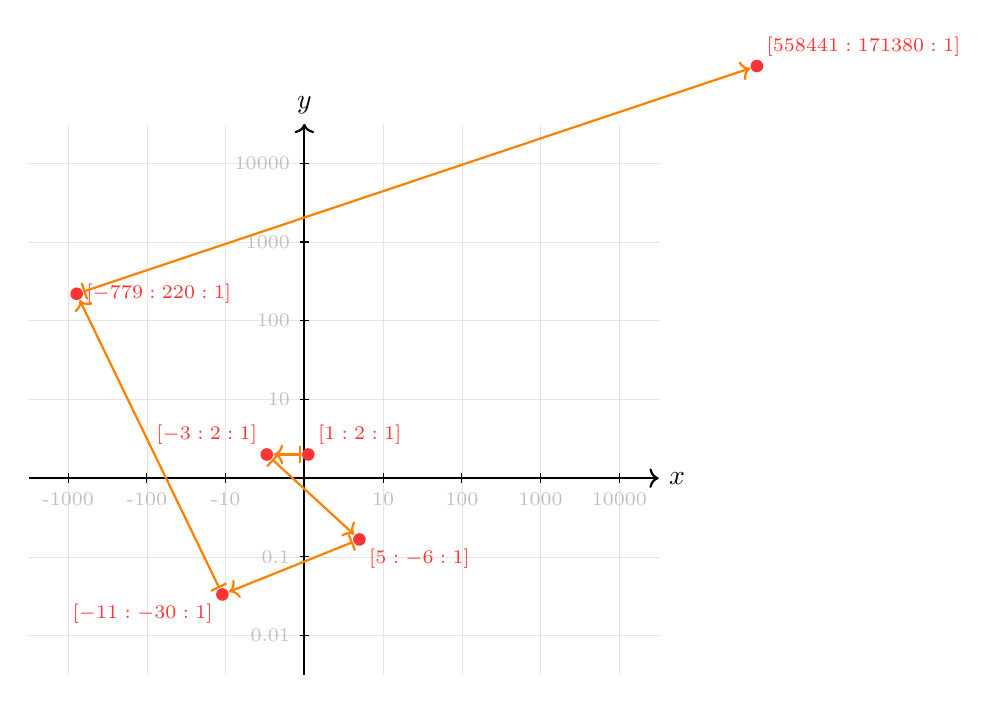
\begin{tikzpicture}
        % axes from -4 to 4 with grid and ticks
        \draw[help lines, gray!20] (-3.5,-2.5) grid (4.5,4.5);
        \draw[->, thick] (-3.5,0) -- (4.5,0) node[right] {$x$};
        \draw[->, thick] (0,-2.5) -- (0,4.5) node[above] {$y$};
        \foreach \pos/\labels in {-3/{-1000}, -2/{-100}, -1/{-10}, 1/{10}, 2/{100}, 3/{1000}, 4/{10000}}{
            \draw (\pos,0.06) -- (\pos,-0.06) node[below,text=gray!50,font=\scriptsize] {\labels};
        }
        \foreach \pos/\labels in {-2/{0.01}, -1/{0.1}, 1/{10}, 2/{100}, 3/{1000}, 4/{10000}}{
            \draw (0.06,\pos) -- (-0.06,\pos) node[left,text=gray!50,font=\scriptsize] {\labels};
        }

        % draw the orbit points and arrows between them
        
        % define named coordinates for the orbit points
        \coordinate (p0) at (0.05,0.301);
        \coordinate (p1) at (-0.477,0.301);
        \coordinate (p2) at (0.699,-0.778);
        \coordinate (p3) at (-1.041,-1.477);
        \coordinate (p4) at (-2.892,2.342);
        \coordinate (p5) at (5.747,5.234);

        % draw the filled points
        \foreach \p in {p0,p1,p2,p3,p4,p5}{
            \fill[red!80] (\p) circle (0.08);
        }

        % draw labels for the points
        \node[above right,font=\scriptsize,text=red!80] at (p0) {\([1:2:1]\)};
        \node[above left,font=\scriptsize,text=red!80] at (p1) {\([-3:2:1]\)};
        \node[below right,font=\scriptsize,text=red!80] at (p2) {\([5:-6:1]\)};
        \node[below left,font=\scriptsize,text=red!80] at (p3) {\([-11:-30:1]\)};
        \node[right,font=\scriptsize,text=red!80] at (p4) {\([-779:220:1]\)};
        \node[above right,font=\scriptsize,text=red!80] at (p5) {\([558441:171380:1]\)};

        % draw arrows between named points
        \draw[|->,thick,orange,shorten <=0.09cm,shorten >=0.09cm] (p0) -- (p1);
        \draw[|->,thick,orange,shorten <=0.09cm,shorten >=0.09cm] (p1) -- (p2);
        \draw[|->,thick,orange,shorten <=0.09cm,shorten >=0.09cm] (p2) -- (p3);
        \draw[|->,thick,orange,shorten <=0.09cm,shorten >=0.09cm] (p3) -- (p4);
        \draw[|->,thick,orange,shorten <=0.09cm,shorten >=0.09cm] (p4) -- (p5);

    \end{tikzpicture}

    \begin{tikzpicture}[remember picture,overlay]
    \node[anchor=south east,xshift=-0.6cm,yshift=0.8cm] at (current page.south east) {%
        \begin{minipage}[c][8cm]{0.44\textwidth}
            {\fontsize{9pt}{11pt}\selectfont
                \setbeamertemplate{itemize item}{\Large\textbullet}
                \begin{itemize}[<+- | alert@+>]
                    \setlength{\itemsep}{8pt}
                    \setlength{\parskip}{2pt}
                    \item 
                    \(X=\mathbb{P}^2\), 
                    
                    \(f:[x:y:z]\mapsto[x^2-y^2:xy:z^2]\),
                    
                    \(x = [1:2:1]\).

                    \item \(f^*H \sim 2H\) \(\implies\) \(\delta_f = 2\).
                    
                    \item 
                    \begin{tabular}{r l l}
                    \(n\) & \(h(f^n(x))\)   &   \\ \hline
                    \(0\) & \(\log 2\)      & \approx \(0.7\) \\
                    \(1\) & \(\log 3\)      & \approx \(1.1\) \\
                    \(2\) & \(\log 6\)      & \approx \(1.8\) \\
                    \(3\) & \(\log 30\)     & \approx \(3.4\) \\
                    \(4\) & \(\log 779\)    & \approx \(6.7\) \\
                    \(5\) & \(\log 558441\) & \approx \(13.2\)
                    \end{tabular}

                    \item It is expected that \(\alpha_f(x) = 2\).

                \end{itemize}
            }
        \end{minipage}
    };
    \end{tikzpicture}

    % Let \(X=\mathbb{P}^2\) and \(f:[x:y:z]\mapsto[x^2-y^2:xy:z^2]\).

    % \(x=[1:2:1]\) has a Zariski dense orbit and \(\delta_f=2\).
    % \(f(x)=[-3:2:1]\), 
    % \(f^2(x)=[5:-6:1]\), 
    % \(f^3(x)=[-11:-30:1]\), 
    % \(f^4(x)=[-779:220:1]\), 
    % \(f^5(x)=[558441:171380:1]\), 

    % log10 coordinates of the orbit points:
    % \((0,0.301),(-0.477,0.301),(0.699,-0.778),(-1.041,-1.477),(-2.892,2.342),(5.747,5.234),\ldots\)

    % Heights:
    % \(h(x)=\log\max\{|1|,|2|,|1|\}=\log2\approx0.7\),
    % \(h(f(x))=\log3\approx1.1\),
    % \(h(f^2(x))=\log6\approx1.8\),
    % \(h(f^3(x))=\log30\approx3.4\),
    % \(h(f^4(x))=\log779\approx6.7\),
    % \(h(f^5(x))=\log558441\approx13.2,\ldots\)
\end{frame}


\begin{frame}{Known cases for KSC}

    \vspace{0.3cm}
    \visible<1->{Projective surfaces                               ([\textcolor{red}{MSS18},\textcolor{red}{MZ22}]);\\
    Quasi-projective surfaces (assuming DML)            ([\textcolor{red}{Wang23}]);\\
    Birational map on surfaces                        ([\textcolor{red}{Xie24}]);\\
    Smooth projective threefolds with \(\deg f>1\)        ([\textcolor{red}{MZ23}]);\\}
    \vspace{1em}
    \visible<2->{Abelian varieties                          ([\textcolor{red}{KS16}]);\\
    Hyperk\"ahler manifolds                           ([\textcolor{red}{LS21}]);\\
    Mori dream spaces                                ([\textcolor{red}{Matsuzawa20}]);\\}
    \vspace{1em}
    \visible<3->{Polarized endomorphisms                      ([\textcolor{red}{KS14}]);\\
    Int-amplified endomorphisms                       ([\textcolor{red}{MZ24}]);\\
    \vspace{1em}
    \(\cdots\)}

\end{frame}


% \begin{frame}{Main results}

%     \vspace{0.5em}

%     \only<1->{
%         % Settings:
%         \textbf{Special Fano fibration case (*)} (as the final output of MMP):\\
%         {\fontsize{10pt}{12pt}\selectfont
%             smooth Fano fibration \(X \xrightarrow{\pi} Y\) of relative Picard number one (\textcolor{green!60!black}{eg. \(\bbP^n\)-bundles}) over 
%             \vspace{-0.8em}
%             \begin{itemize}
%                 \item[(*1)] an abelian variety; or
%                 \item[(*2)] a smooth projective variety of Picard number one.
%             \end{itemize}
%             \vspace{-1em}
%         }

%         \only<7-8>{\alert<7>{
%             \vspace{0.2em}
%             \textbf{Dynamical conditions (\(\dagger\))}: \\
%             {\fontsize{10pt}{12pt}\selectfont
%                 the fibration \((X,f)\xrightarrow{\pi} (Y,g)\) does not preserve the dynamical degree, i.e., \(\delta_f > \delta_g\);\\
%                 if in the case (*2), we further require \(\delta_g = 1\).\\
%             }
%         }}
%     }

%     \only<2-6>{
%         \vspace{1em}
%         \begin{theorem}[{[Meng-Wang-Y]}]\label{thm: mainthm}
%             KSC holds for \(X\) in the special Fano fibration case (*).
%         \end{theorem}
%     }

%     \only<3-4>{
%         \vspace{0.5em}
%         \visible<3->{Consider \(f \acts X\).
%         After iteration, the dynamics \(f \acts X\) descends to \(g \acts Y\),} 
%         \visible<4->{i.e., there is a commutative diagram
%         \[\begin{tikzcd}[ampersand replacement=\&]
%             X \arrow{r}{f} \arrow{d}{\pi} \& X \arrow{d}{\pi} \\
%             Y \arrow{r}{g} \& Y.
%         \end{tikzcd}\]}
%     }

%     \only<5-6>{
%         \vspace{0.5em}
        

%         \visible<5-6>{If \alert{\(\delta_f = \delta_g\)}, then 
%         \vspace{-0.6em}
%         \begin{center}
%             \begin{tabular}{@{}l@{}}KSC for abelian varieties \\ or polarized endomorphisms\end{tabular} \(\implies\) KSC for \((Y,g)\) \(\implies\) KSC for \((X,f)\). 
%         \end{center}}

%         \visible<6>{In the \alert{case (*2)}, if \alert{\(\delta_g > 1\)}, then \(f\) is int-amplified and KSC holds by {[Meng-Zhong24]}.}
%     }

%     \only<8>{
%         \begin{theorem}[{New Fibration, [Meng-Wang-Y]}]
%             \vspace{0.5em}
%             In the special Fano fibration case (*) with dynamical conditions (\(\dagger\)), there exists an equivariant fibration
%             \[ f \acts X \overset{\varphi_{f,R_f}}{---\!\twoheadrightarrow} Z \racts h \]
%             with \(\dim Z>0\) and \(h\) is \(\delta_f\)-polarized (in particular, \(\delta_h = \delta_f\)).
%         \end{theorem}
%     }

% \end{frame}

\begin{frame}{Main results}

    \vspace{0.5em}

    % Settings:
    \textbf{Special Fano fibration case (*)} (as a final output of MMP):\\
    {\fontsize{10pt}{12pt}\selectfont
        smooth Fano fibration \(X \xrightarrow{\pi} Y\) of relative Picard number one (\textcolor{green!60!black}{eg. \(\bbP^n\)-bundles}) over 
        \vspace{-0.8em}
        \begin{itemize}
            \item[(*1)] an abelian variety; or
            \item[(*2)] a smooth projective variety of Picard number one.
        \end{itemize}
        \vspace{-1em}
    }

    \visible<3->{\alert<3>{
        \vspace{0.2em}
        \textbf{Dynamical conditions (\(\dagger\))}: \\
        {\fontsize{10pt}{12pt}\selectfont
            the fibration \((X,f)\xrightarrow{\pi} (Y,g)\) does not preserve the dynamical degree, i.e., \(\delta_f > \delta_g\);\\
            if in the case (*2), we further require \(\delta_g = 1\).\\
        }
    }}

    \only<2>{
        \vspace{1em}
        \begin{theorem}[{[Meng-Wang-Y]}]\label{thm: mainthm}
            KSC holds for \(X\) in the special Fano fibration case (*).
        \end{theorem}
    }

    \only<4>{
        \begin{theorem}[{[Meng-Wang-Y]}]
            \vspace{0.5em}
            In the special Fano fibration case (*) with dynamical conditions (\(\dagger\)), there exists an equivariant fibration
            \[ f \acts X \overset{\varphi_{f,R_f}}{---\!\twoheadrightarrow} Z \racts h \]
            with \(\dim Z>0\) and \(h\) is \(\delta_f\)-polarized (in particular, \(\delta_h = \delta_f\)).
        \end{theorem}
    }

\end{frame}


\begin{frame}{Sketch of proof}
    \vspace{1em}
    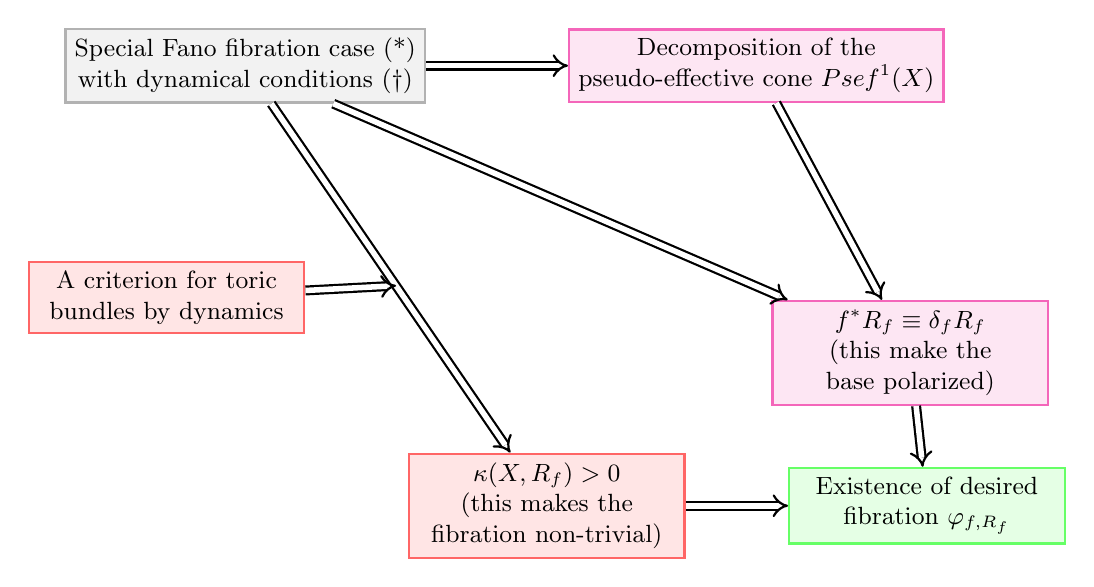
\begin{tikzpicture}[
        node distance=0.5cm and 0.8cm,
        every node/.style={font=\small},
        box/.style={rectangle, draw=blue!60, fill=blue!5, thick, minimum width=3.5cm, minimum height=0.8cm, align=center},
        graybox/.style={rectangle, draw=gray!60, fill=gray!10, thick, minimum width=3.5cm, minimum height=0.8cm, align=center},
        magentabox/.style={rectangle, draw=magenta!60, fill=magenta!10, thick, minimum width=3.5cm, minimum height=0.8cm, align=center},
        redbox/.style={rectangle, draw=red!60, fill=red!10, thick, minimum width=3.5cm, minimum height=0.8cm, align=center},
        assumption/.style={rectangle, draw=red!60, fill=red!10, thick, minimum width=3.5cm, minimum height=0.8cm, align=center},
        conclusion/.style={rectangle, draw=green!60, fill=green!10, thick, minimum width=3.5cm, minimum height=0.8cm, align=center},
        contradiction/.style={rectangle, draw=orange!80, fill=orange!15, thick, minimum width=3.5cm, minimum height=0.8cm, align=center},
        arrow/.style={->,>=Stealth,thick},
        implies/.style={-Implies,double,double distance=2pt,thick}
    ]
        % Nodes
        \visible<1->{\node[graybox] (settings) {Special Fano fibration case (*) \\ with dynamical conditions (\(\dagger\))};}

        \visible<2->{\node[magentabox, right=of settings, xshift=1cm] (decomp) {Decomposition of the \\ pseudo-effective cone \(\Psef^1(X)\)};}

        \visible<3->{\node[magentabox, below right=of decomp, yshift=-2cm, xshift=-3cm] (eigenvector) {\(f^*R_f \equiv \delta_f R_f\)\\(this make the\\base polarized)};}

        \visible<4->{\node[redbox, below=of settings, yshift=-1.5cm, xshift=-1cm] (toric) {A criterion for toric \\ bundles by dynamics};}

        \visible<5->{\node[redbox, below right=of toric,xshift=0.5cm,yshift=-1cm] (positivity) {\(\kappa(X,R_f) > 0\)\\ (this makes the\\fibration non-trivial)};}

        \visible<6->{\node[conclusion, right=of positivity,xshift=0.5cm] (result) {Existence of desired \\ fibration \(\varphi_{f,R_f}\)};}

        % Arrows
        \visible<2->{\draw[implies] (settings) -- (decomp);}
        \visible<3->{\draw[implies] (decomp) -- (eigenvector);}
        \visible<3->{\draw[implies] (settings) -- (eigenvector);}

        % \visible<2->{\draw[implies] (start) -- (logetale);}
        \visible<5->{\draw[implies] (settings) -- (positivity);}
        \visible<5->{\draw[implies] (toric) -- ($(settings)!0.5!(positivity)$);}

        \visible<6->{\draw[implies] (eigenvector) -- (result);}
        \visible<6->{\draw[implies] (positivity) -- (result);}

    \end{tikzpicture}

\end{frame}


% ----------------------------------------------------------

% Thank you slide
{
    \setbeamertemplate{background}{}
    \begin{frame}[plain]

    \vspace{0.2\textheight}
    \Huge{\centerline{\textbf{\alert{Thank You!}}}}

    \vfill
    \centerline{\includegraphics[width=0.35\textwidth]{\ECNULibThanks}}
    \end{frame}
}


\end{document}